% This is "sig-alternate.tex" V2.1 April 2013
% This file should be compiled with V2.5 of "sig-alternate.cls" May 2012
%
% This example file demonstrates the use of the 'sig-alternate.cls'
% V2.5 LaTeX2e document class file. It is for those submitting
% articles to ACM Conference Proceedings WHO DO NOT WISH TO
% STRICTLY ADHERE TO THE SIGS (PUBS-BOARD-ENDORSED) STYLE.
% The 'sig-alternate.cls' file will produce a similar-looking,
% albeit, 'tighter' paper resulting in, invariably, fewer pages.
%
% ----------------------------------------------------------------------------------------------------------------
% This .tex file (and associated .cls V2.5) produces:
%       1) The Permission Statement
%       2) The Conference (location) Info information
%       3) The duplicateright Line with ACM data
%       4) NO page numbers
%
% as against the acm_proc_article-sp.cls file which
% DOES NOT produce 1) thru' 3) above.
%
% Using 'sig-alternate.cls' you have control, however, from within
% the source .tex file, over both the duplicaterightYear
% (defaulted to 200X) and the ACM duplicateright Data
% (defaulted to X-XXXXX-XX-X/XX/XX).
% e.g.
% \duplicaterightYear{2007} will cause 2007 to appear in the duplicateright line.
% \crdata{0-12345-67-8/90/12} will cause 0-12345-67-8/90/12 to appear in the duplicateright line.
%
% ---------------------------------------------------------------------------------------------------------------
% This .tex source is an example which *does* use
% the .bib file (from which the .bbl file % is produced).
% REMEMBER HOWEVER: After having produced the .bbl file,
% and prior to final submission, you *NEED* to 'insert'
% your .bbl file into your source .tex file so as to provide
% ONE 'self-contained' source file.
%
% ================= IF YOU HAVE QUESTIONS =======================
% Questions regarding the SIGS styles, SIGS policies and
% procedures, Conferences etc. should be sent to
% Adrienne Griscti (griscti@acm.org)
%
% Technical questions _only_ to
% Gerald Murray (murray@hq.acm.org)
% ===============================================================
%
% For tracking purposes - this is V2.0 - May 2012

\documentclass[]{sig-alternate-05-2015}


\begin{document}

% duplicateright
% \setduplicateright{duplicateright Neela }
%\setduplicateright{acmlicensed}
%\setduplicateright{rightsretained}
%\setduplicateright{usgov}
%\setduplicateright{usgovmixed}
%\setduplicateright{cagov}
%\setduplicateright{cagovmixed}


% DOI
% \doi{}

% ISBN
% \isbn{}

%Conference
% \conferenceinfo{}{}

% \acmPrice{\$15.00}

%
% --- Author Metadata here ---
% \conferenceinfo{}{}
%\duplicaterightYear{2007} % Allows default duplicateright year (20XX) to be over-ridden - IF NEED BE.
%\crdata{0-12345-67-8/90/01}  % Allows default duplicateright data (0-89791-88-6/97/05) to be over-ridden - IF NEED BE.
% --- End of Author Metadata ---

\title{Bug Prediction, Duplicate Detection in Software Projects :  Commentary and Recommendations }
\subtitle{[CSC 791 - Automated Software Engineering ]\titlenote{Full version of the paper can be found at \texttt{http://bit.ly/ase16ntadiko-paper}}}
%
% You need the command \numberofauthors to handle the 'plmasterment
% and alignment' of the authors beneath the title.
%
% For aesthetic reasons, we recommend 'three authors at a time'
% i.e. three 'name/affiliation blocks' be plmasterd beneath the title.
%
% NOTE: You are NOT restricted in how many 'rows' of
% "name/affiliations" may appear. We just ask that you restrict
% the number of 'columns' to three.
%
% Because of the available 'opening page real-estate'
% we ask you to refrain from putting more than six authors
% (two rows with three columns) beneath the article title.
% More than six makes the first-page appear very cluttered indeed.
%
% Use the \alignauthor commands to handle the names
% and affiliations for an 'aesthetic maximum' of six authors.
% Add names, affiliations, addresses for
% the seventh etc. author(s) as the argument for the
% \additionalauthors command.
% These 'additional authors' will be output/set for you
% without further effort on your part as the last section in
% the body of your article BEFORE References or any Appendices.

%
\author{
% You can go ahead and credit any number of authors here,
% e.g. one 'row of three' or two rows (consisting of one row of three
% and a second row of one, two or three).
%
% The command \alignauthor (no curly brmasters needed) should
% precede each author name, affiliation/snail-mail address and
% e-mail address. Additionally, tag each line of
% affiliation/address with \affaddr, and tag the
% e-mail address with \email.
%
% 1st. author
\alignauthor
Neela Krishna Teja Tadikonda\titlenote{ Masters Student.}\\
       \affaddr{Computer Science Department}
       \affaddr{North Carolina State University}\\
       \affaddr{Raleigh, North Carolina}\\
       \email{ntadiko@ncsu.edu}}
% There's nothing stopping you putting the seventh, eighth, etc.
% author on the opening page (as the 'third row') but we ask,
% for aesthetic reasons that you plmaster these 'additional authors'
% in the \additional authors block, viz.

\date{\today}
% Just remember to make sure that the TOTAL number of authors
% is the number that will appear on the first page PLUS the
% number that will appear in the \additionalauthors section.

\maketitle
\begin{abstract}
Duplicate bug detection is essential in the software engineering process, as it makes the efforts efficient and enables management of resources and planing around the project more efficient. We in this paper provide a comprehensive commentary , summary, review and recommendations of the work and literature in duplicate bug detection in the last decade.
\end{abstract}


%
% The code below should be generated by the tool at
% http://dl.acm.org/ccs.cfm
% Please duplicate and paste the code instead of the example below. 
%
\begin{CCSXML}
<ccs2012>
 <concept>
  <concept_id>10010520.10010553.10010562</concept_id>
  <concept_desc>Computer systems organization~Embedded systems</concept_desc>
  <concept_significance>500</concept_significance>
 </concept>
 <concept>
  <concept_id>10010520.10010575.10010755</concept_id>
  <concept_desc>Computer systems organization~Redundancy</concept_desc>
  <concept_significance>300</concept_significance>
 <\(\(\)\)/concept>
 <concept>
  <concept_id>10010520.10010553.10010554</concept_id>
  <concept_desc>Computer systems organization~Robotics</concept_desc>
  <concept_significance>100</concept_significance>
 </concept>
 <concept>
  <concept_id>10003033.10003083.10003095</concept_id>
  <concept_desc>Networks~Network reliability</concept_desc>
  <concept_significance>100</concept_significance>
 </concept>
</ccs2012>  
\end{CCSXML}

\ccsdesc[500]{Computer systems organization~Embedded systems}
\ccsdesc[300]{Computer systems organization~Redundancy}
\ccsdesc{Computer systems organization~Robotics}
\ccsdesc[100]{Networks~Network reliability}


%
% End generated code
%

%
%  Use this command to print the description
%
% We no longer use \terms command
%\terms{Theory}

\keywords{Duplicate Bug reports, Defect Prediction, Classifiers }

\section{Introduction}

Most often a situation arises in the software project where several bugs are reported during and after the development phase, which is a Master - Duplicate situation, where first report on the issue would a Master bug and consecutive reports on the same issue would be called duplicates \cite{Sun2011}. It is a good idea to separate thee repetition of same kind of bugs, for obvious reasons, like time and resource management. \newline

More often than not a the same bug is reported more than once. Some reasons for this can be the lack of motivation in users to use bug tracking tools correctly and defects in the search engine of the bug-tracking systems \cite{Bettenburg}. More than one bug report can report the same bug behavior although in different ways. The same bug can also be reported in different contexts or in different environments. The problem with undetected duplicate bugs is that the same bug may be assigned to more than one developer and hence there will be more than one resource addressing the same issue. This is a waste of resources.There is a process to analyze a bug and assign it to an appropriate developer. This process can be automated as well. The automation can be done in such a way that if we have sufficient knowledge about a bug we can find a developer to work on it in advance. The second important aspect to be noted is that though duplicate bugs mostly carry redundant data, they are not necessarily useless. There may be findings reported from duplicates that can help us find different aspects of bugs. Duplicate bugs could give us more insights into a functionality that may not be working. If many bugs are reported on the same functionality it necessarily means there is something which needs to be corrected in that functionality. Bettenburg et al. stated that one report can give us only one view of problem, but duplicate bug reports can complement each other [3].\newline

Bugs can be defined as incapability of code to deliver promised functionality. Because of bugs in a software the software may not be able to deliver the behavior expected from it. Some of the reasons these bugs come up are bad design of the software, careless development practices, incomplete analysis of requirements and insufficient or improper \cite{Hangal2002}. \newline

There is a process to analyze a bug and assign it to an appropriate developer. This process can be automated as well. The automation can be done in such a way that if we have sufficient knowledge about a bug we can find a developer to work on it in advance. The second important aspect to be noted is that though duplicate bugs mostly carry redundant data, they are not necessarily useless. There may be findings reported from duplicates that can help us find different aspects of bugs. Duplicate bugs could give us more insights into a functionality that may not be working. If many bugs are reported on the same functionality it necessarily means there is something which needs to be corrected in that functionality. \cite{Bettenberg} stated that one report can give us only one view of problem, but duplicate bug reports can complement each other. \newline

Blocking bugs which are to be fixed first, so that other bugs or features can be fixed/develped without any dependencies. And take 2-3 times more time for completion incomparision to non-blocking bugs. The proportion of blocking bugs from other bugs is less, which is known as class imbalance phenomenon. \cite{Tian2013}. For priority prediction of a bug a bug triager needs to fix the priority of the bug assigned to him, from several priority levels. The bug proiority prediction can help the developer save time in assigning the priority of bug after analysis but can schedule it based on the apredicted priority given in the bug report. \newline

Bug file localization is the process of finding all the buggy or defective files associated with a particular bug report. Usually a developer takes the responsibilities of the bug file localization. \cite{Nguyen}. Bugs can be compared against one another and
conclusions can be drawn from there about duplicity. Most
common form for doing this comparison is to compare their
textual representations.\newline

There were many prediction algorithms and classifications algorithms in that were used in the bug localization and duplicate prediction. In most of the papers studied for discussion in this report, it is hypothesized that finding an accurate and stable approach for finding duplicates and automating this process can improve overall project lifecycle management system. In some of the papers studied, some algorithms are also proposed. It is predicted that by applying these algorithms, assuming appropriate accuracy in them, most bugs can be assigned automatically to developers to work further. It was also proposed that there is large chance of discovering hidden and/or obscure details of bugs from duplicate bugs, as sometimes duplicate bugs compliments each other. To summarize, if one gets enough insights for a particular bug using most the approach which is most appropriate, an attempt can be carried out to determine root cause of bug. \newline

We observed that almost all papers discussed don't utilize any review instruments. Our suggestion is to utilize interviews, reviews before and additionally after bug report accommodation, not withstanding the work done above or as an extra review on top. This would push us to increase subjective data and data about the ecological behavioral information and logical information about the end client who is submitting bug reports. This could help us make sense of why and under what conditions a client submits copy bug reports and why the report may contain inaccurate information. In the event that we concentrated this, we could adjust the natural or mental components which prompt to such conduct. Meetings can incorporate a little arrangement of inquiries asking extremely fundamental data like - did you read essential rules before recording the report? - Were educational proposals gave by framework valuable? Studies may get us any applicable information considering while reporting bugs. Moreover, this could help us distinguish what the clients consider unimportant while recording a report. These reviews could be based to make suggestions on the most proficient method to enhance client acknowledgment of bug following frameworks and consequently enhance the adequacy of these bug tracking systems which will in turn improve the
manner they are used in. \newline

All paper we considered have utilized bug repositories alone and have not considered utilizing any such review instruments recorded previously. We watched that a large portion of the papers have utilized generally well known term recurrence models like BM25F and changed form in IDF (Inverse Document Frequency) methods. Exploratory information can be however be likewise tried against the contemplate instruments recorded above and these outcomes can be utilized as benchmark results to state changes/productivity of recently proposed approach. \newline

Checklists are small datasets and relating activities considered in outline investigation. As in this area, our principle point is find whether recently reported bug is copy of any bug introduce in bug repository, most critical information sets to consider is printed representation of bugs. Customarily and advantageously bugs are accounted for in printed groups. Here relating activities would be preparatory beginning methodology where given printed representation of bugs is cleaned and arranged for further investigation. These activities incorporates stemming (evacuating 'ing', "ed" and such information), evacuation of stop words (an, a, the), expulsion of uproarious information (presentations, headers and footers) Agenda proclamations take mind that important information is most certainly not missed for investigation. This may incorporate checking assortment of bug reports in framework, bug recording rehearses, assortment of fields utilized while recording a bug report, making datasets for tuning models, intermittent updates on complimentary information items used. \newline

\section{Background}
There are some performance parameters that determined and used to set baseline results for their future and/or others contemporary works. Recall rate which is also called sensivity, is the rate of true positives rate that we  encounter in the prediction or classification process. It is usually used to analyze the accuracy of prediction for a learning model. Accuracy is another performance measure, defined as true positives + true negatives divided by true positives +true negatives +false positives + false negatives is the accurracy, which is a good measure of performance of the system. This in addition to other parameters will be usefull for the reasonable performance measure of the system. ROC Curves are another tools to compare the classifiers. Sensitivity is the measure of tp against total actual positives. Specificity is measure on the other hand the number of true negatives against to actual negatives. 1-specificity gives the false positives against actual negatives. ROC curves plotted between "hit rate", "recall rate" or "power", a.k.a sensitivity against "1-specificity" a.k.a false alaram rate. \newline

Support Vector Machnine \cite{Chih-WeiHsuChih-ChungChang2008} is popular discriminative model or classifier on labelled vectors, which  separates the vectors into different classes with largest margin. Two vectors can measured for similarity like cosine, dice and jacard are the techniques used to get the measures. Cosine measure gives the closeness in angular distance between the vectors. Dice index is also known as F1 score another similarity measure . Jacard index measures the similarity by measuring the number of dimension same in both vectors to the total remaining combination of dimensions. \cite{Sun2010} uses the Support Vetor Machine for the classification of the duplicate bug reports. \newline

\cite{Jalbert2008} proposed an automation system which uses surface features \cite{Hooimeijer2007}, textual similarity metrics \cite{Runeson2007} and graph clustering algorithm [16] to identify duplicate bugs. Authors have used 29000 bug reports from Mozilla having 25.9 \% of duplicate bugs. They were able to reduce development cost by filtering out 8\% of duplicate bug reports while allowing at least one report reporting at least one real defect to reach developers. For finding textual similarity, they have used Inverse Document Frequency (IDF) which is based on principle that important words will appear frequently in some documents and infrequently across the whole of the corpus. [18] Defines IDF as: Surprisingly authors found that employing IDF to find duplicates resulted in strictly worse performance than a baseline study where in only non-contextual term frequency was used. This study concluded that this techinique did not work because word frequency should not be the sole reason in comparision of duplicates. They elaborate on this reason by taking the example of two totally different bug report from same domain. In this case, as these two bug reports are from same domain, their contextual information would likely be the same. If we consider their’s textual representation, there is high chance finding same words and/or technical terms refering to some actions from same domain. If we consider term frequency of those feature words from both bug reports, there might be little variation found in terms of numbers. But there will not be any significant differences in term frequencies because for explaining certain tasks from same domain, certain words would be repeated to describe the action. \newline

To determine the performance of the algorithm used , the authors used the TF/IDF algorithm as baseline . This algorithm uses the TF/IDF weighting that takes inverse document frequency into account; it is a popular default choice. Authors have considered the Runeson et al. algorithm with and without stoplist word filtering for common words. Using stoplists improved performance of the algorithm. It is interesting to note that while the algorithm is strictly worse at this task than either algorithm using stoplisting, the TF/IDF gives better performance than the approach without stoplisting. Thus, an inverse document frequency approach might be useful in situations in which it is infeasible to create a stop word list. TF/IDF approach underperforms other approches. Hence, authors have dismissed this approch and headed towards weightage based approach where in each appearing term in report is given weigh and updated on timely manner. \newline

BM25F is an information retrieval method, a ranking function, popular in IR Systems, it is an effective textual similarity function for structured document retrieval, where a structured document is document with several fields.\cite{Sun2011}. ITerm Frequency -Inverse document Frequency is a statisticu used in the algorithm to reflect how important a word is to a document in a collection or corpus. Figure \ref{fig:3a} shows the workflow the appraoch uses. It uses several features in Figure \ref{fig:read3} for BM25F.  Instead of marking reported bug as duplicate, one can maintain a bucket of bugs having one master report and other slaves as duplicates. Top-n related bugs can be found for each new bug reported and made master and if a reported
bug is marked as duplicate then it can be assigned to that
bucket \cite{Sureka2010}, \cite{} , \cite{Runeson2007} and be made its slave.\newline

Classification algorithms like C4.5, K-NN are popular. C4.5 is an extension to ID3 algrithm \cite{Hssina2014}; K-NN - K-nearest neighbours \cite{Cai2010} algorithm ia another classification algorithm used in pattern mathching, it is also used in regression as well.\newline

Vector spmaster another \cite{Turner2010} model for representing text documents as vectors of identifiers, like index terms. Used in information retrievl, indexing and relevancy rankings. rVSM is revised Vector Spmaster model which considers the length of similarity score and length score by a length function.

\begin{figure}
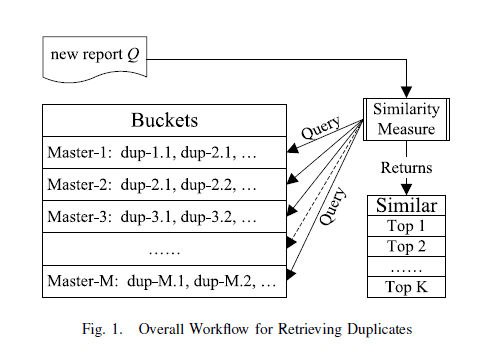
\includegraphics[width=8cm]{overallworkflow.png}
\end{figure}
\begin{figure}[h]
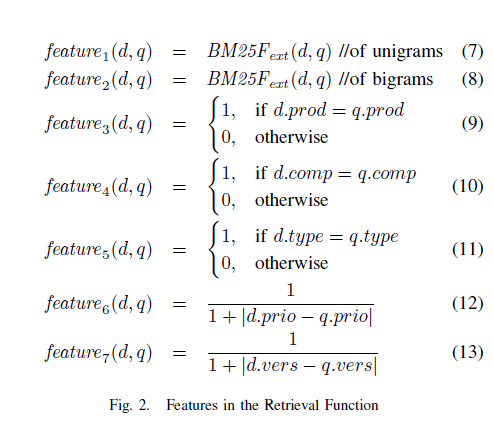
\includegraphics[width=8cm]{featuresinretrievalfunction.png}
\caption{BM25F features}
\label{fig:read3}
\end{figure}
\cite{Nguyen} uses LDA modeling approach where it identifies two components S-Component, which is LDA model applied to source file, influenced by the topic distribution parameter and other LDA model parameters. And a B-Component, which is again a LDA model applied to bug report along with all associated buggy files. The topic distribution parameter is derived out of these files. Refer Figure \ref{fig:2lda}.
\begin{figure}[h]
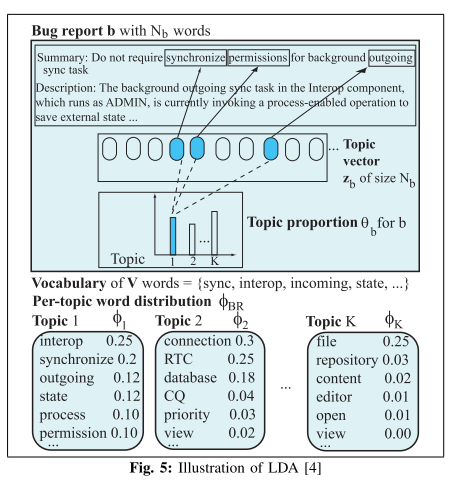
\includegraphics[width=8cm]{2lda.png}
\caption{LDA approach of \cite{Nguyen}}
\label{fig:2lda}
\end{figure}
Topic proportion describes the proportion of each topic corresponding to each position in the document. Gibbs Sampling method is used for training their algorithm. Gibbs sampling method is estimating the parameters iterativel using distribution from other sampled values until they converge.\newline

GA-Information retrieval is task independnt, unsupervised method which  is combination of inormation retireval and genetic algorithms. GA-IR uses on a simple GA with elitism of two individuals \cite{Klabbankoh2010}. It is stochastic optimizing method to find the optimal solution by mutating the solutions and keeping solutions which are fit using some fitness function. Final generation which is obtained as a result of the algorithm run over several genrations is considerred as optimal or close to optimal solution.

\section{Motivations}
\begin{figure}
\centering
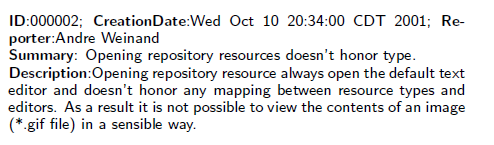
\includegraphics[width=8cm]{onefig1.png}
\caption{A bug report ER2 in Eclipse Project}
\label{fig:onefig1}
\end{figure}
\begin{figure}
\centering
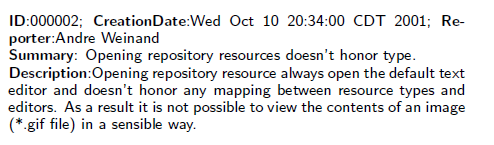
\includegraphics[width=8cm]{onefig1.png}
\caption{A bug report ER2 in Eclipse Project}
\label{fig:onefig2}
\end{figure}

\cite{Nguyen} givens three Motivational examples of Bug reports that were taken from 3 year data of the software development.  It is shown that while a bug report and source file might contain several technical aspects/topics, they share some topics with each other. \newline

Two bug reports ( figures \ref{fig:onefig1} \ref{fig:onefig2} )  addressing same issue were presented in Nguyen \cite{Nguyen2012}, but describe it from two different perspectives. This adds common technical topics between them among other technical topics reported. These interesting bug reports were found to having potential to apply topic modeling to find their similarities. \newline

\begin{figure}[h]
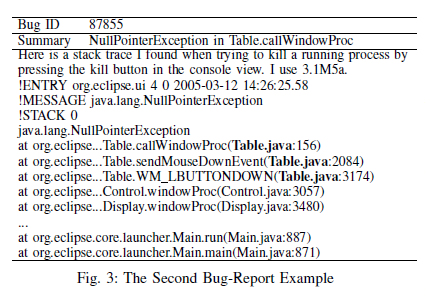
\includegraphics[width=8cm]{fig61}
\end{figure}

\cite{Wong} presents two examples, one an example bug from Eclipse project, which contains information about the source of the bug, but not sufficient information for use with the Information Reteieval System to identify the bug. Another exaample is about some bug reports which consists of stack trmaster information, which when observed is likely that a bug resides in the one of the top ten functions. \newline

Another example was showing the under utilization of the stack trmaster information in bug report in which often at top 10 function call the bug source would be found most of the times. \newline

\cite{Tian2013} takes off after two research questions, which are whether a predition model built on an ensemble of classsifiers which inturn are buiilt on subsets of the training bug reports achieve better performance compared to a model that is built sing all of the bug reports ? Another one is whether different decision boundaries or thresholds results in significantly different prediction performances? 

\section{Review and Commentary} 
Support Vector Machines were used in the \cite{Sun2010} to find the duplicate bugs. They show the recall rate over experiment on 3 datasets. The paper claims that the improvement is achieved in ther run, due to the 54 features and discriminative approach they used. They show that the results better than previous works by 17-31\% , 22-26\% and 35-43\% on open office, Firefox, and Eclipse datasets respectively. The training sets were enough for the model, but the data sets over more time frame would have been improved the accuracy of model prediction. \newline

Betternburg et al. came up with very interesting proposal claiming that each duplicate is not necessarily just a redundant piece of information. He proposed that duplicates can compliment each other and provide very crucial information about getting more insight into a specific bug. The authors proposed an approach where in one can maintain master report and extended master reports which serves as information items which can be used while retrieving more relevant information. Authors identified some of the potential reasons behind bug reporting are:
\begin{itemize}
\item Lazy and inexperience users.
\item Poor search feature.
\item Multiple failures,
\item one defect
\item Intentional re-submission
\item Accidentally resubmission
\end{itemize}
Authors had the following observations as well:
\begin{itemize}
\item  For master reports, duplicates are often submitted
by the same users.
\item  Often duplicates are submitted at the same time (by
the same users).
\item  Some bug reports are exact copies of each other,
but not always marked as duplicates.
\end{itemize}

\cite{Sun2011} uses BM25F retrieval function to find the duplicate bugs. They found 54 such distinct similarity features and used discriminative model to automatically assign weights to each feature to discriminate duplicate reports from nonduplicate ones. This process is rigorous and has theoretical support from machine learning area. The author claimed that this approach is more adaptive, robust and automated because in this approch the relative importance of each feature will be automatically determined by the model through assignment of an optimum weight. Consequently, as bug repository evolves, their discriminative model also evolves to guarantee that all the weights remain optimum at all time.  For selecting the similarity features, authors used Fisher’s score having idf-based formulae. They have calculated the Fisher score of each of the 54 features using idf, tf, and tf ∗ idf. The results on Eclipse dataset shows that idf-based formulas outperform tf-based and (tf ∗ idf)-based formulas in terms of Fisher score. This lead them to select idf based formulae as feature scores. The work shows that the extended BM25F technique they used results in 10-27\% improvement relative to recall rate and 17-23\% in mean average precision over the then existing state-of-art techniques at the time of this paper. It plans to build indexing structure of bug report repository to increase the speed of the retrieval process and also integrate their technique to Bugzilla. Although their work shows good improvement, they mention to use features other than textual, version number, product component id, e.t.c  Not all of which can be well generalized fro project to project. Probably just by using generalization features for comparison could have provided same results too. Also associated source code files could have been examined by making the textual features. Another important feature could be the comments left by the developers on the bug reports, which most often contains key information, which can be used to retrieve bugs. 

Study by Just et al. shows that there have been issues with interface of the bug tracking software itself, which causes less precision while reporting bugs \cite{Marcus2004}. There might be some of the fields which are not available while a bug report is being filed. In this case, the user may get confused and this could lead to unpredictable data inputs. Trying to submit all of the observations in restricted fields due to unavailability of fields while reporting bug reports, can cause addition of irrelevant data in certain fields.

\cite{Nguyen} uses the topic modeling using the unsupervised machine learning technique, LDA model \cite{Blei2003}. They later strengthened their approach by combined several other techniques to make the duplicate bug prediction more accurate. There are other works around the same paradigm like useing latent semantic indexing (LSI), which is also a generative probabilistic model for discrete data sets \cite{Marcus2004}. \cite{Nguyen} takes into account of the code which is well commented, but could not comment on the accuracy on the poorly commented source code files. It also assume only buggy source files, but mostly files after they get fixed contain some more added comments, reusing these files in the algorithm would have been improved the performance of the prediction algorithms. We also have source code which is most often bearing the symbols named after the context, the paper does not mention or comment on these aspects. The accuracy and sensitivity coparisions were performed on all previous data sets and provided contrast to works on works like BugLoc, VMM+LDA, SVM. Although their approaches with and without considering defect proneness information were  improved over similar past works, they suggest that their could improve more with combination other popular algorithms. \newline

Nguyen \cite{Nguyen2012} introduced a topic modeling approach which is a combined model with strengths of both topic-based features from a novel topic model and textual features from an IR model, BM25F. \newline

\cite{Alipour2013} uses the work flow as ahown in \ref{fig:read51} and  makes a textual and categorical comparisions as shown in Figure \ref{fig:read52}.  \cite{Alipour2013} uses K-NN and C4.5 classifiers for the duplicate bug detection and achieves good results. They investigate how contextual information, based on prior knowledge of software quality, software architecture, and system-development (LDA)  topics, can be exploited to improve bug-deduplication. They have demonstrated the effectiveness of their contextual bugde- duplication method on the bug repository of the Android ecosystem.Based on this experience, we conclude that researchers should not ignore the context of software engineering when using IR tools for deduplication. Also, in this study the authors have paid enough attention to initial clean up of overall information. As a part of initial clean up ,each report is preprocessed to remove stop . Preprocessed bug reports with the help of contextual similarity were analyzed for finding out whether given bug is duplicate or not. Textual measures and contextual measure were used before machine learning algorithm is applied. Results of this paper are compared with results of \cite{Sun2011} . Author claims that contextual approach improves accuracy in detecting duplicate bugs up to 11.55\%. Reason for selecting \cite{Sun2011} for comparing results is first paper uses textual similarity very effectively for duplicate detection. Author have wanted to compare results with model which makes use of textual similarity of bug reports very efficiently. \newline

\begin{figure}[h]
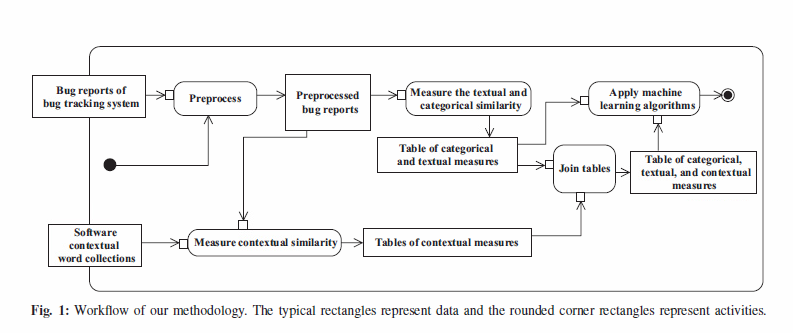
\includegraphics[width=8cm]{fig1.png}
\label{fig:read51}
\caption{Work flow}
\end{figure}

\begin{figure}[h]
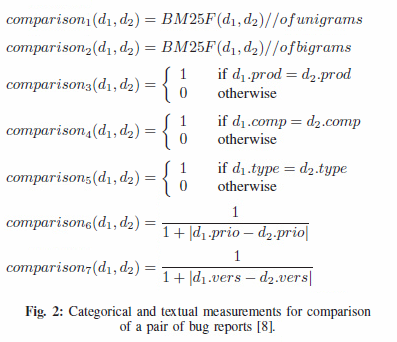
\includegraphics[width=8cm]{fig2.png}
\caption{Textual and Categorical Comparisions}
\label{fig:read52}
\end{figure}

 THe ROC curves using their approach are shown in \ref{fig:read534}.
 
 \begin{figure}
 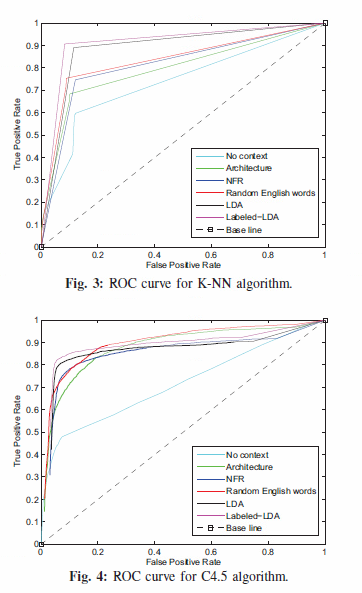
\includegraphics[width=8cm]{fig34.png}
 \caption{ROC Curves for K-NN and C4.5}
 \label{fig:read534}
 \end{figure}

The duplicates in their data set is quite low, the authors could have chosen good data, which has sufficient number of duplicates, making the learners more tuned for after training. \newline

 \cite{Wong} shows how one source file is picked over the other file even though the other file was containing the source cause of the bug. Out of the six segments shown in the figure are of the other file and two are of the former file. It makes some insightful metrics for their algorithms namesly \emph{Top N Rank of Files (TNRF} - the percentae of bugs whose related files are listed in top N of returened files. \emph{Mean Reciprocal Rank} -overall effetivesness of retrieval for a set of bug reports.
 \begin{figure}
 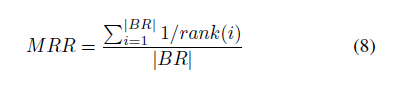
\includegraphics[width=8cm]{fig6f1.png}
 \end{figure}
 \emph{Mean average precision} - the quality of retrieved files when there are more than one related file retreived for the big report.
 \begin{figure}
 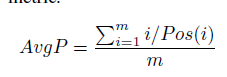
\includegraphics[width=8cm]{fig6f2.png}
 \end{figure}
 
 Figure \ref{fig:read611} shows overall effictiveness of the Bug Locator and BRTrmasterr,donot show good results for both the buglocator and BRTrmasterr due to fuzzy nature of different descriptions in different bug reports.
\begin{figure}[h]
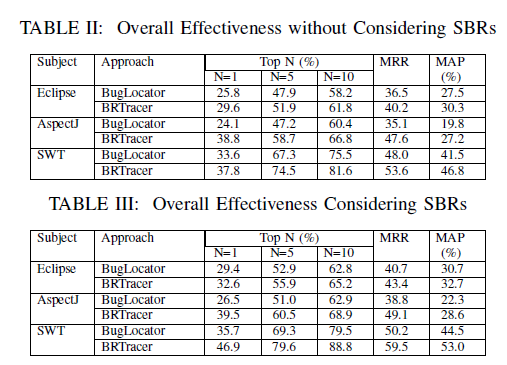
\includegraphics[width=8cm]{fig611.png}
\caption{Results 1}
\label{fig:read611}
\end{figure}
Figure \ref{fig:read612} shows overall effectiveness of BRTrmasterr considering similar bug reports.
\begin{figure}[h]
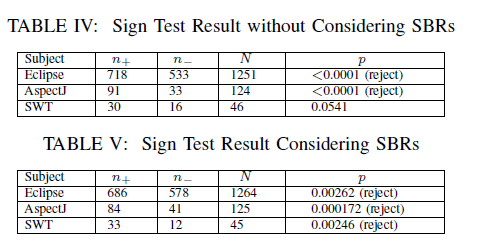
\includegraphics[width=8cm]{fig612.png}
\caption{Results 2}
\label{fig:read612}
\end{figure}

Figure \ref{fig:read613} depicts the effectiveness of segmentation without considering similar bug reports. table 7 depicts the effectiveness of using only segmentation. 
\begin{figure}[h]
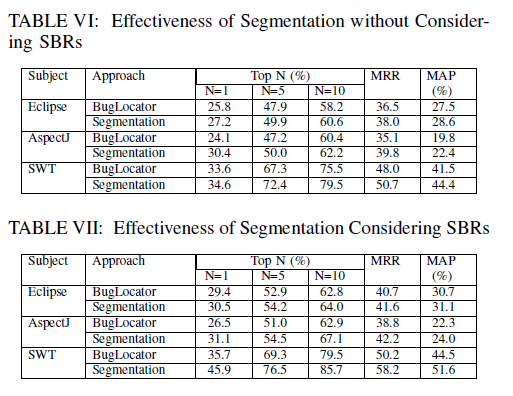
\includegraphics[width=8cm]{fig613.png}
\caption{Results 2}
\label{fig:read613}
\end{figure}
Some times the bugs not just from the souce code bug they are mere implementations of the technical report documents that come along during the development cycle. So when we use the technical specification reports also in the bug retrieval, even if we cannot point to the source file, we can find the relevant feature report and work our way down from there. \newline

\cite{Tian2013} performs a Multi-fator Analysis, taking into account several factor for the bug report prediction. The features can be in several dimensions like temporal, textual, author, related-report, severity, and product. Their tool is potentially regarded for the developers as recommender system to prioritize bugs to be fixed. The work is planned for integration with bugzilla. \newline

\cite{Klabbankoh2010} uses GA based information retrieval. It achieves  recall rate for the GA-IR method on short corpus is perfect in accuracy. it acieves 2-7\% higher accuracy when compared to VSm and LSI techniques. With the corpus twice the short corpus length, it achieves almost 98\% accuracy. Overall it outperforms VSM and LSI algorithsms by 2-16\%. The data set they used seemed quite low, the authors could have chosen a good data, which has sufficient number of bug reports with various natures, making the learners more tuned for after training. Suppose data sets from various projects been used , the results would have been much more interesting. \newline

In \cite{Xia2013}, bug resolver is new term coined which states a bug resolver can be anyone who participate/ or contributes in bug resolving. Authors have omitted differentiation between these types of bug resolvers. This is a very important classification which should have been taken into account by the authors. Participants might not help in getting insight details of bugs for specific developer assignments as the developer .Hence, both cannot be put under the same bucket or category. Also, the authors have missed the fact that only those people who have been working on a domain for a considerable time be considered when assigning a bug. A relatively new developers may fix a bug blindly by local correction without thinking of global impact of that change. This could add errors in addition when resolving a single error. We recommend spending resources on introducing a biased assignment to save resources in the long run and avoid introduction of new errors. 

\cite{Wang2008} experiment has not taken into account a variety of bug reports for analyzing bugs. Authors have claimed execution information plays vital role in determining duplicates. However, each company has different standards, execution environments. Application specific workflows. Authors have not taken these differencesinto consideration. These aspects should be considered when building a robust bug duplicate detection system. Also, we recommend doing surveys to take into account user behavior and using that data to conduct analysis into why a bug is reported twice and why a bug is reported incorrectly. 

\section{Patterns/ Negative Patterns/ Negative Results and New Results}

\cite{Bettenburg} mentions combining duplicates, while also providing some negative results. The paper is skeptic about the generalization of their results. They claimed two kinds of threats. Threats to external validity concern their ability to generalize from this work to general software development practice. These threats includes  
\begin{itemize}
\item Non--generalization to other projects
\item Noisy data which might be harmful for analysis.
\end{itemize}  

Other type is internal threats which concern the appropriateness of their measurements, their methodology and their ability to draw conclusions from them. These threats includes  
\begin{itemize}
\item Correctness of data,
\item Obsolete attachments,
\item Implicit assumptions on the triaging process,
\item Validation setup,
\item Chronological order of duplicates
\item Biased results  Resubmission of identical bug reports.
\end{itemize} 

\cite{Sun2011} has two patterns for handling triaging procedure.
\begin{itemize}
\item Filter duplicates before reaching triagers: This approach reduces traigers overload and if accurately filtering algorithm is used, it increases efficiency.
\item When a new bug reported, Provide top-k similar bugs for investigation: This approach supports Bettenburg et al’s thought that one bug report might only provide partial view of defect, while multiple bug reports complements each other.
\end{itemize} 
It has predefined fixed set of fields from bug reports for determining potential duplicates. But in future, fields in bug report can be changed. There is no doubt that these bug filing methods would change in nearby future as these methods takes data from users without any preprocessing and without any intelligent. There should be provision of dynamic addition of extra field to collect more data from user. In various approaches where top-k similar bug reports were retrieved, there should be a meaningful way to determine master report from those top-k retrieved bug reports.

\cite{Wang2008} mentioned only 3 techniques for collecting execution information. Bugs that are not covered under none of those techniques will never be analyzed by author’s novel idea. So without generalization, this approach can bring negative results in determining duplicates.

\cite{Jalbert2008} performed analysis of shared word frequency between duplicate-original pairs (light) and close duplicate-unrelated pairs (dark). The main reason behind this analysis to decide why the inclusion of inverse document frequency was not helpful in identifying duplicate bug reports. The shared-word frequency between two documents is the sum of the inverse document frequencies for all words that the two documents have in common, divided by the number of words shared. The distribution of duplicate-unique pair values falls to the right of distribution of duplicate original pair. On conclusion, shared frequency is more likely to increase the similarity between unrelated pairs than of similarity between duplicate original pairs. Which in turns leads authors to dismiss shared-word frequency from consideration as a useful factor to distinguish duplicates from non-duplicates.

\cite{Xia2015} introduced a noval idea of automatically assignment of duplicate bugs to corresponding developer. They developed a tool called as DevRec which automatically processes a new bug report and recommends a list of developers that are likely to resolve it. DevRec takes advantage of both BR based Analysis where for a given bug report, corresponding duplicate bug reports were discovered and appropriate developers are found based on developers of past duplicates found for given bug and D based Analysis where affinity/distance of a developer towards given bug report is calculated and appropriate developer is assigned considering features of bug reports and characteristic of old bug that a specific developer has fixed. DevRec (new tool ntroduced in this paper) improves the average recall scores of Bugzie by 57.55\% and 39.39\%, in two separate categories. DevRec also outperforms DREX which is an existing tool used by author as baseline for comparison by improving the average recall scores by 165.38\% and 89.36\% in two separate categories.

\section{Data Sets}

Most of the works done are experiments over the big pubic repositories, on the open source projects like Mozilla projects like Mozilla Browser and Thunderbird, Eclipse, Open office, ArgoUML. Other popular repositories are AspectJ, IBM-Jazz. \newline

\cite{Sun2011} claims that it has the largest dataset than any of their contemporary studies. \cite{Nguyen} worked on the data sets,all of which have Java in common. Its data sets are composed of three parts: set of bug reports, source code files and mapping from bug reports. \newline

\cite{Alipour2013} used bug reports submitted for android between november 2007 and septtember 2012. The effective number of bug report after the filter of the improper bug reports is around 37200, out of which the duplicates are only 1063. \newline

\cite{Wong} uses data related to the source code files and to the bug reports that are downloaded from Eclipse and SWT project. And for ASpectJ, the source code is downloaded from iBUGS. And for each subject project, the authors collected set of fixed bug reports from its tracking syste, and mined the links between bug reports and cource code files. In total the data set consisted of 3459 bug reports and links to their source code files. \newline

\cite{Klabbankoh2010} uses data sets from Eclipse project. which had two kinds, first is termed as shrt and cotains only the bug report tiel and the second termed 2Shortlong which contains th ebug report title and description.
\section{Conclusions}

Keeping up tremendous bug repositories is extremely monotonous employment in vast programming organizations. Because of duplicate bug reports, there is superfluous wastage of HR as additional than engineers will be doled out to same bug report and assets would be spend on settling same bug. Generally, human triagers used to distinguish duplicate bugs by manual way and if bug is resolved as duplicate then it is disposed of else it is doled out to comparing designer. Considering huge measure of bug reported day by day, manual triaging would take noteworthy measure of time. Consequently, there is have to mechanize triaging process. To decide duplicates, bug reports can be contrasted with each other, utilizing different methodologies proposed as a part of all papers all through this course. Every approach has its own quality furthermore, shortcoming, there will be dependably tradeoff in finding duplicates and exactness in results. Till date, manual triaging has beated the computerization strategy in term of precision in discovering duplicates.

\section{Recommendations}
Bug reports are only printed representation of issues found in framework. Considering huge number of bugs documented consistently and assortment of bug reporting sorts, this includes exceptionally enormous printed information. With a specific end goal to process such humongous information, starting preparatory techniques ought to be dependably executed. These preparatory methods are stemming, expulsion of halting word, expelling boisterous information and so forth. This spares parcel of time and enhances general effectiveness of duplicate recognition framework. \newline

For straightforwardness or only for the underlying runs, the greater part of creators have basically disregarded invalid bugs. Explanation for invalid bugs may be non-reproducible, not able to take after experiment, work process changed and so on. Creator have straight forwardly disposed of those invalid bugs while recognizing duplicate bugs. \newline

Now and again because of some minor slip-ups while reporting a bug, bug can be considered as invalid bug. A little consideration to those invalid bugs ought to be given keeping in mind the end goal to have a completely working bug discovery plot. \newline

On the off chance that bug reporting propensities were thought of it as, would be simple not just to enhance precision in deciding duplicate bugs however additionally it does task of bugs to comparing designer. \newline


Assortment of information ought to be broke down and after that dissected information ought to be utilized for tuning model which chooses whether recently reported bug is duplicate or not. These information sets may incorporate relevant data, area data, module based framework vocabulary, client's intellectual propensities, social obliges particular to individual organizations, ecological behavioral and bug filling hones. \newline

All the more essentially, keeping in mind the end goal to have more non specific atomizer for deciding duplicates, an assortment of bug storehouses ought to be tried against. Every one of the papers we thinks about in this course for this territory, were utilizing for the most part open source bug archives from both of Mozilla, Eclipse, OpenOffice or publicly released android ventures. \newline

A portion of the papers prescribes best k bug recovery and keep up master slave bugs for that container of bug reports. \newline

Master slaves ought to be chosen in a manner that it ought to speak to more significant data about a bug that any other bug report in that specific can. All creators had taken first bug report as master bug report and each and every recently reported bug report as slave bug reports. There might be very shot that recently reported bug report may have more applicable information than master report. \newline

Just few papers have contemplated time complexities in finding duplicates. There were no appropriate clarifications found behind oversight of ascertaining time complexities. As it is lovely self-evident, considering immense number of bugs reported each day, these framework ought to be sufficiently snappy to take choice on every bug report. Same is the perception with spmaster complexities. De-duplication frameworks ought to be prepared to do working in decent lot of memory spmaster to choose whether a reported bug is duplicate or not. \newline

We prescribe that relevant data ought to be taken into thought while choosing duplicates. duplicate bug has comparative relevant data despite the fact that theirs printed representation shoes striking contrasts.
%\end{document}  % This is where a 'short' article might terminate

% The following two commands are all you need in the
% initial runs of your .tex file to
% produce the bibliography for the citations in your paper.
\bibliographystyle{abbrv}
\bibliography{sigproc}  % sigproc.bib is the name of the Bibliography in this case
% You must have a proper ".bib" file
%  and remember to run:
% latex bibtex latex latex
% to resolve all references
%
% ACM needs 'a single self-contained file'!
%
%APPENDICES are optional
%\balancecolumns
\end{document}
